\section{Unsupervised learning}
\begin{itemize}
	\item We can express our data distribution by marginalizing latent variables (unobserved targets/values that make it easier to understand the data). This allows us to model the data with more tractable joint distributions with simpler components to understand:
	\begin{equation*}
		\begin{split}
			\bm{z}\text{ continuous: } & p\left(\bm{x}\right) = \int p\left(\bm{x}, \bm{z}\right) d\bm{z} = \int p\left(\bm{x}| \bm{z}\right) p\left(\bm{z}\right)d\bm{z}\\
			\bm{z}\text{ discrete: } & p\left(\bm{x}\right) = \sum\limits_{\bm{z}} p\left(\bm{x}, \bm{z}\right) = \sum\limits_{\bm{z}} p\left(\bm{x}| \bm{z}\right) p\left(\bm{z}\right)\\
		\end{split}
	\end{equation*}
	\item Discrete latent variables are typically used for clustering, whereas continuous are applied for dimensionality reduction 
\end{itemize}
\subsection{\textit{K}-means Clustering}
\begin{itemize}
	\item Every single data point $\bm{x}$ is assigned to a cluster $\to$ a discrete latent variable $\bm{z}$
	\item Number of clusters/different values for $\bm{z}$ must be determined beforehand
	\item Cluster as comprising a group of data points whose inter-point distances are small compared with the distances to points outside the cluster
	\item Hence, we define $\bm{\mu}_k$ as a prototype (here also the mean) of the cluster $k$, and minimize the sum of squares of the distances of each data point to its closest vector $\bm{\mu}_k$:
	$$J=\sum\limits_{n=1}^{N}\sum\limits_{k=1}^{K} z_{nk} ||\bm{x}_n - \bm{\mu}_k||^2$$
	where $\bm{z}_n$ is a one-hot vector with $z_{nk}=1$ if $k$ is closest cluster of $\bm{x}_n$
	\item Optimization algorithm (expectation-maximization (EM) algorithm):
	\begin{enumerate}
		\item Means $\bm{\mu}_k \in \mathbb{R}^D$ are initialized randomly
		\item Repeat until convergence ($\mu_k$ and $z_{nk}$ do not change for any $n$ and $k$):
		\begin{enumerate}
			\item \textbf{Expectation step}: Find the assignment of the closest cluster for every data point:
			$$\frac{\partial J}{\partial z_{nk}}=0 \Rightarrow z_{nk} = \begin{cases}
			1 & \text{ if } k=\arg\min\limits_j ||\bm{x}_n - \bm{\mu}_j||^2\\
			0 & \text{ otherwise }
			\end{cases}$$
			\item \textbf{Maximization step}: Find the means of each cluster:
			$$\frac{\partial J}{\partial \bm{\mu}_{k}}=0 \Rightarrow \bm{\mu}_k = \frac{\sum_n z_{nk}\bm{x}_n}{\sum_n z_{nk}}$$
		\end{enumerate}
	\end{enumerate}
	\begin{figure}[ht]
		\centering
		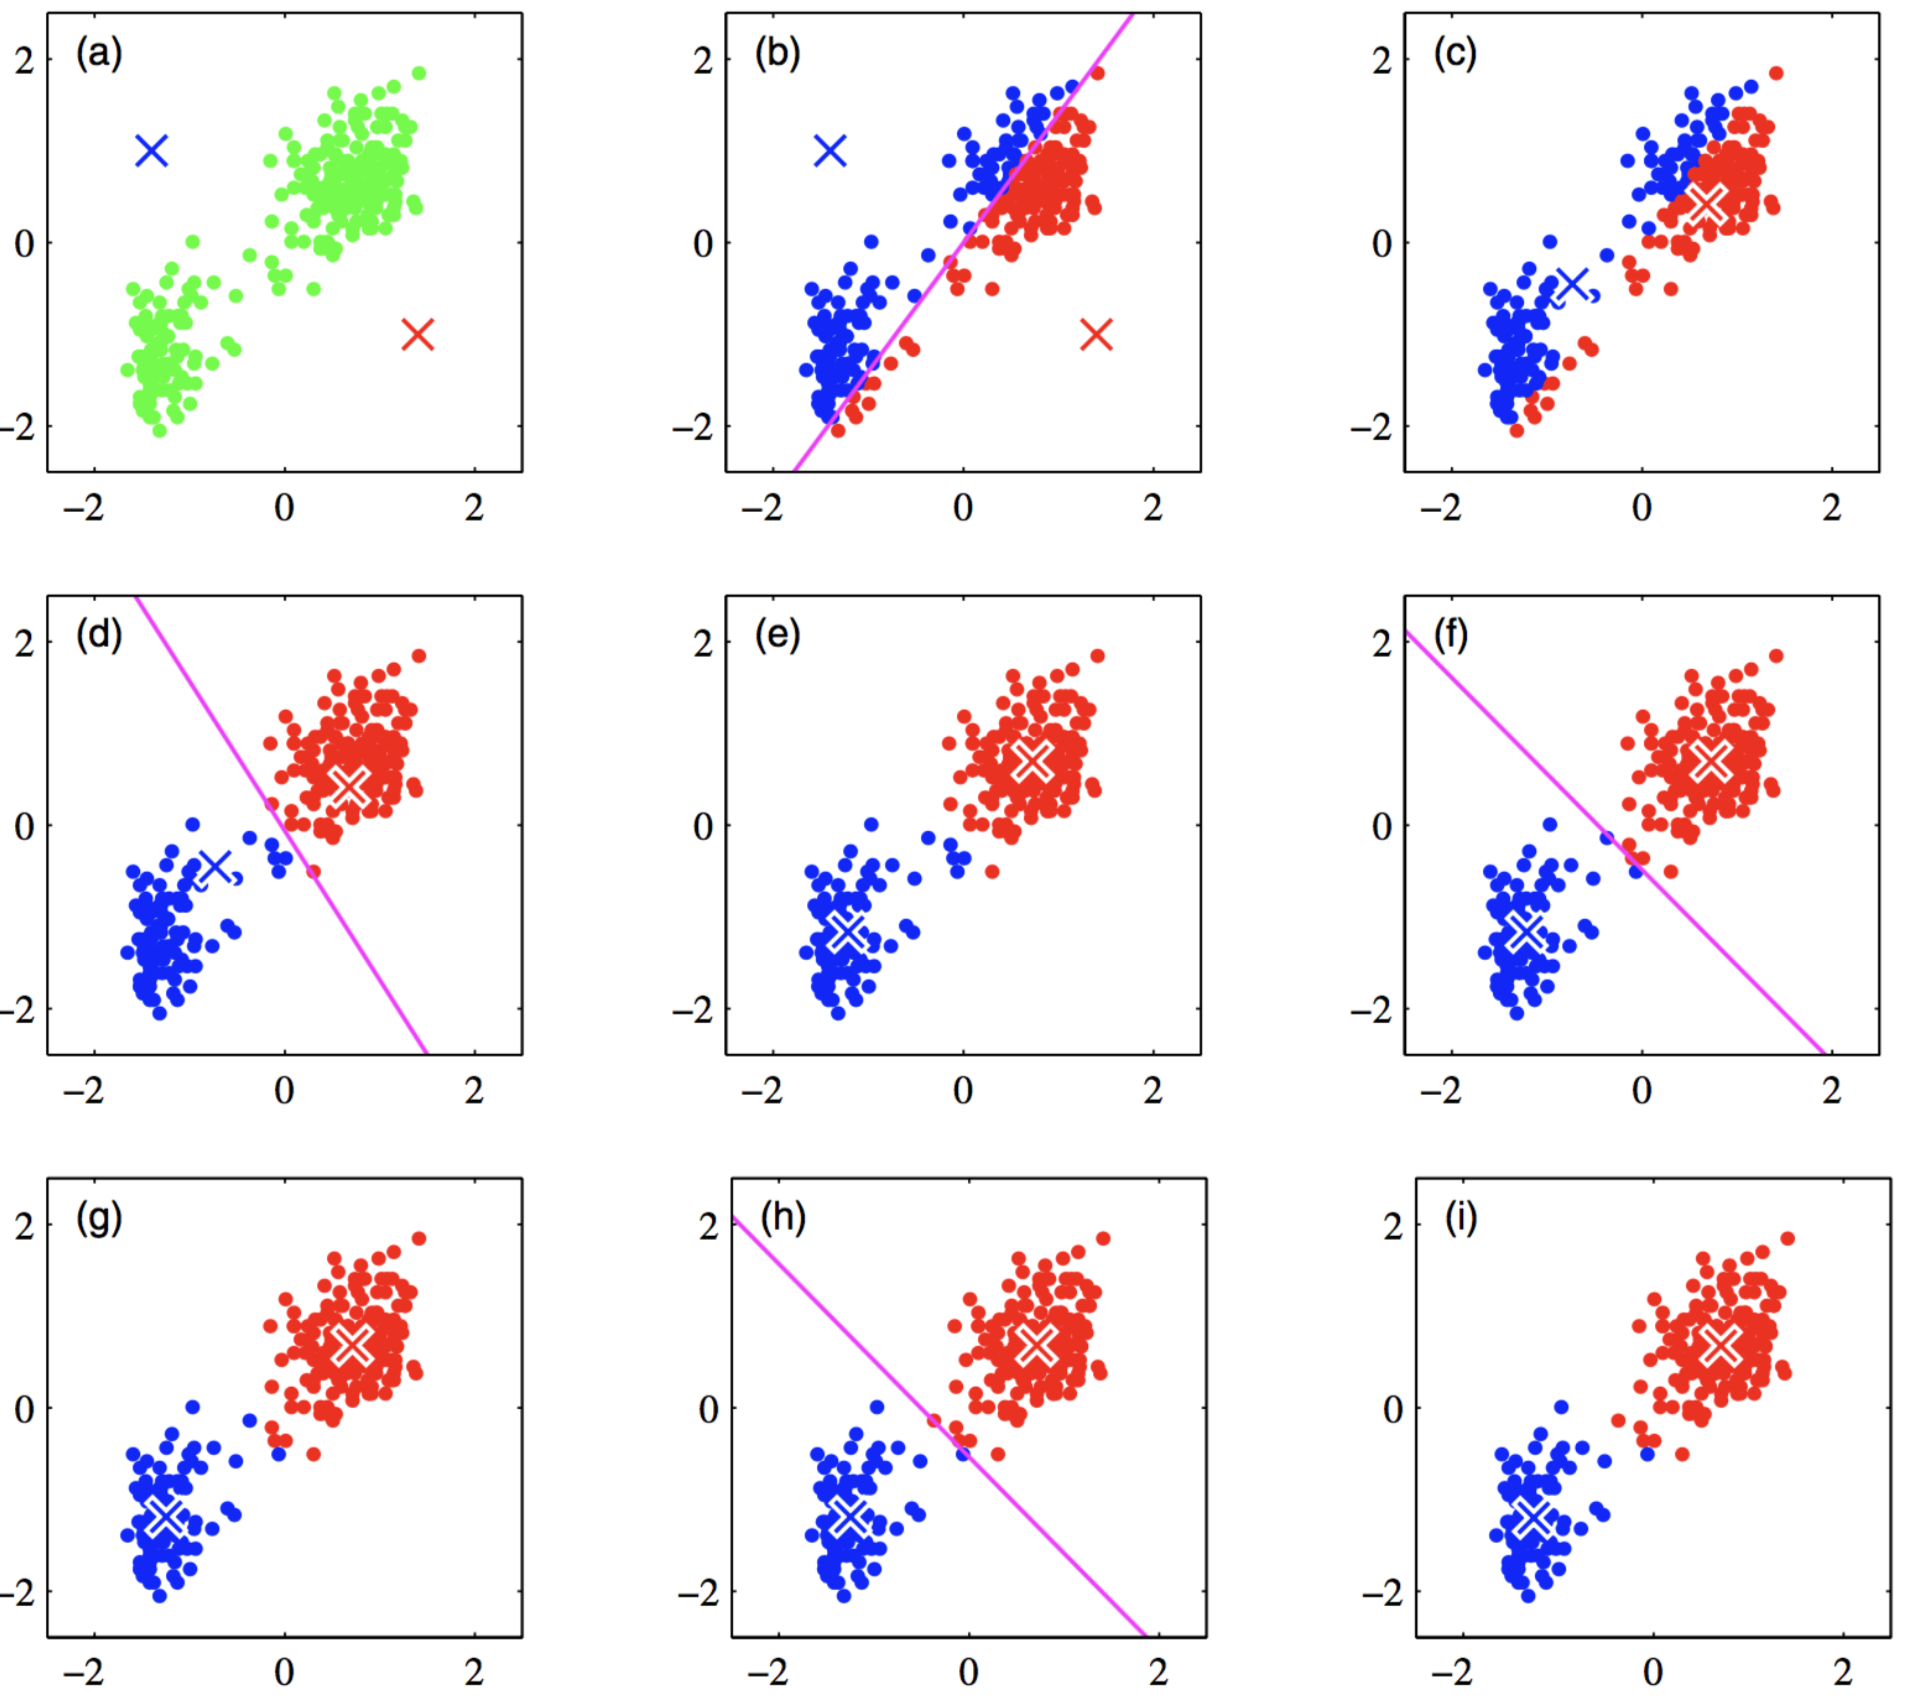
\includegraphics[width=0.4\textwidth]{figures/k_means_example.png}
		\caption{Illustration of the $K$-means algorithm. First, an expectation step is performed where the data points are assigned to a cluster (see \textit{(b)}, \textit{(d)}, \textit{(f)}, and \textit{(h)}), and then the maximization step optimizes the means of the clusters (see \textit{(c)}, \textit{(e)}, \textit{(g)}, and \textit{(i)}).}
		\label{img:k_means_example}
	\end{figure}
	\item The algorithm converges as each phase reduces the value of the objective function $J$, but they might converge to a local rather than global minimum (perform multiple random restarts and choose best minimum found)
	\item \textbf{Application}: image compression. Every pixel is a data point, and we search for $K$ clusters representing different colors in the image. The image is compressed by only using the cluster means (colors) instead of specifying a color at every pixel. A problem of this method is that the position correlations are ignored.
	\item \textbf{Failures} of $K$-means:
	\begin{itemize}
		\item $K$-means is only able to cluster spherical data due to the squared distance we try to minimize. Other shapes require different distance measures or data transformation by some basis functions.
		\item $K$-means strongly prefers clusters of the same size/spread, and therefore tries to find cluster with the same spread in the dataset.
		\item $K$-means is very sensitive to outliers. As it tries to minimize the squared distance, outliers may have a significant effect on the cluster means.
	\end{itemize}
	\item \textbf{Improvements}:
	\begin{itemize}
		\item For a large dataset, we can use SGD to reduce computational effort. The update for a single data point would look like:
		$$\bm{\mu}_k^{(\tau+1)} = \bm{\mu}_k^{(\tau)} - \eta \left(\frac{\partial J}{\partial \bm{\mu}_k^{(\tau)}}\right)^T = \bm{\mu}_k^{(\tau)} + 2 \eta \left(\bm{x}_n - \bm{\mu}_k^{(\tau)}\right)$$
		\item Use other distance measure between points that is for example not so sensitive to outliers:
		$$\tilde{J} = \sum\limits_{n=1}^{N}\sum\limits_{k=1}^{K} z_{nk} \mathcal{V}\left(\bm{x}_n, \bm{\mu}_k\right)$$
		where $\mathcal{V}$ measures the similarity of $\bm{x}_n$ and $\bm{\mu}_k$.
	\end{itemize}
	\item \textbf{Pros and cons} of $K$-means
	\begin{itemize}
		\item[+] Simple to implement
		\item[+] Fast
		\item Local minima
		\item Only models spherical data 
		\item Sensitive to feature scales and outliers
		\item Number of clusters $K$ must be specified in advance with prior knowledge
		\item Cluster assignments are hard and not probabilistic
	\end{itemize}
\end{itemize}
\subsection{Mixture of Gaussians and EM algorithm}
\begin{itemize}
	\item Approximate the joint distribution $p\left(\bm{x},\bm{z}\right)=p\left(\bm{x}|\bm{z}\right)\cdot p\left(\bm{z}\right)$ by a mixture of Gaussians ($\bm{z}$ chooses the mixture component, and points in the cluster are Gaussian distributed)
	\item We define the prior as $p\left(z_k=1\right)=\pi_k$, where $\sum_k \pi_k= 1$ and $\pi_k \in [0,1]$
	\item The single clusters are Gaussian: $p\left(\bm{x}|z_k=1\right) = \mathcal{N}\left(\bm{x}|\bm{\mu}_k, \bm{\Sigma}_k\right)$
	\item Overall, the generative distribution is $p\left(\bm{x}\right) = \sum_{k=1}^{K} \pi_k \mathcal{N}\left(\bm{x}|\bm{\mu}_k, \bm{\Sigma}_k\right)$
	\item The posterior/conditional probability of $\bm{z}$ given $\bm{x}$ is also defined as the \textit{responsibility} (that component $k$ in the mixture model takes for 'explaining' the observation/data point $\bm{x}$):
	$$p\left(z_k=1|\bm{x}\right) = \frac{p\left(\bm{x}|z_k=1\right)\cdot p\left(z_k=1\right)}{\sum_j p\left(\bm{x}|z_j=1\right)\cdot p\left(z_j=1\right)}=\frac{\pi_k \mathcal{N}\left(\bm{x}|\bm{\mu}_k, \bm{\Sigma}_k\right)}{\sum_j \pi_j \mathcal{N}\left(\bm{x}|\bm{\mu}_j, \bm{\Sigma}_j\right)} = \gamma\left(z_{k}\right)$$
	\item To optimize our parameters, we again maximize the log-likelihood:
	$$\ln p\left(\bm{X}|\bm{\pi}, \bm{\mu}, \bm{\Sigma}\right) = \sum\limits_{n=1}^{N} \ln \sum\limits_{k=1}^{K} \pi_k \mathcal{N}\left(\bm{x}|\bm{\mu}_k, \bm{\Sigma}_k\right)$$
	\item However, maximizing the log-likelihood has no closed-form solution as stationary points depend on $\gamma\left(z_{nk}\right)$ which again depends on $\bm{\pi}, \bm{\mu}$ and $\bm{\Sigma}$ $\Rightarrow$ use expectation maximization algorithm by alternating the update of (\textit{expected}) posterior $\gamma\left(z_{nk}\right)$ and \textit{maximizing} for parameters $\bm{\pi}, \bm{\mu}$ and $\bm{\Sigma}$
	\item Maximizing with respect to $\bm{\mu}_k$:
	\begin{equation*}
		\begin{split}
			& \frac{\partial}{\partial \bm{\mu}_k} \sum\limits_{n=1}^{N} \ln p\left(\bm{x}_n|\left\{\pi_k\right\}_{k=1}^{K}, \left\{\bm{\mu}_k\right\}_{k=1}^{K}, \left\{\bm{\Sigma}_k\right\}_{k=1}^{K}\right)\\
			= & \sum\limits_{n=1}^{N} \frac{1}{ p\left(\bm{x}_n|\left\{\pi_k\right\}_{k=1}^{K}, \left\{\bm{\mu}_k\right\}_{k=1}^{K}, \left\{\bm{\Sigma}_k\right\}_{k=1}^{K}\right)} \frac{\partial}{\partial \bm{\mu}_k} p\left(\bm{x}_n|\left\{\pi_k\right\}_{k=1}^{K}, \left\{\bm{\mu}_k\right\}_{k=1}^{K}, \left\{\bm{\Sigma}_k\right\}_{k=1}^{K}\right)\\
			= & \sum\limits_{n=1}^{N} \frac{\pi_k \mathcal{N}\left(\bm{x}_n|\bm{\mu}_k, \bm{\Sigma}_k\right)}{\sum\limits_{j=1}^{K}\pi_j \mathcal{N}\left(\bm{x}_n|\bm{\mu}_j, \bm{\Sigma}_j\right)} \left(\bm{x}_n - \bm{\mu}_k\right)^T\bm{\Sigma}_k^{-1}\\
			= & \sum\limits_{n=1}^{N} y\left(z_{nk}\right) \left(\bm{x}_n - \bm{\mu}_k\right)^T\bm{\Sigma}_k^{-1}\\
			\Rightarrow & \bm{\mu}_k = \frac{\sum_{n=1}^{N}\gamma\left(z_{nk}\right)\bm{x}_n}{\sum_{n=1}^{N}\gamma\left(z_{nk}\right)}
		\end{split}
	\end{equation*}
	\item For maximizing $\pi_k$ we need to use the Lagrange multiplier (as the sum must be 1):
	\begin{equation*}
		\begin{split}
			& \frac{\partial}{\partial \pi_k} \sum\limits_{n=1}^{N} \ln p\left(\bm{x}_n|\left\{\pi_k\right\}_{k=1}^{K}, \left\{\bm{\mu}_k\right\}_{k=1}^{K}, \left\{\bm{\Sigma}_k\right\}_{k=1}^{K}\right) + \lambda \left(\sum\limits_{j=1}^{K}\pi_j - 1\right)\\
			= & \sum\limits_{n=1}^{N} \frac{\pi_k \mathcal{N}\left(\bm{x}_n|\bm{\mu}_k, \bm{\Sigma}_k\right)}{\sum\limits_{j=1}^{K}\pi_j \mathcal{N}\left(\bm{x}_n|\bm{\mu}_j, \bm{\Sigma}_j\right)} + \lambda \pi_k\\
			= & \sum\limits_{n=1}^{N} \gamma\left(z_{nk}\right) + \lambda \pi_k\\
			\Rightarrow & \pi_k = -\frac{1}{\lambda}\sum\limits_{n=1}^{N} \gamma\left(z_{nk}\right)\\[10pt]
			& \frac{\partial}{\partial \lambda} \sum\limits_{n=1}^{N} \ln p\left(\bm{x}_n|\left\{\pi_k\right\}_{k=1}^{K}, \left\{\bm{\mu}_k\right\}_{k=1}^{K}, \left\{\bm{\Sigma}_k\right\}_{k=1}^{K}\right) + \lambda \left(\sum\limits_{j=1}^{K}\pi_j - 1\right)\\
			= & \sum\limits_{j=1}^{K}\pi_j - 1 = -\frac{1}{\lambda}\sum\limits_{n=1}^{N} \underbrace{\sum\limits_{j=1}^{K}\gamma\left(z_{nj}\right)}_{=1} - 1 = 0\\
			\Rightarrow & \lambda = -N, \pi_k = \frac{N_k}{N} \text{\hspace{5mm}where\hspace{5mm}} N_k = \sum\limits_{n=1}^{N} \gamma\left(z_{nk}\right) \text{\hspace{2mm}(effective number of points in \textit{k})}
		\end{split}
	\end{equation*}
	\item Maximizing $\bm{\Sigma}_k$ is done by:
	$$\bm{\Sigma}_k = \frac{1}{N_k} \sum\limits_{n=1}^{N} \gamma\left(z_{nk}\right)\left(\bm{x}_n - \bm{\mu}_k\right)^T\left(\bm{x}_n - \bm{\mu}_k\right)$$
	\item Summarized EM algorithm steps for Gaussian mixture models: 
	\begin{itemize}
		\item \textbf{Expectation step}: update the posterior:
		$$\gamma\left(z_{k}\right) = \frac{\pi_k \mathcal{N}\left(\bm{x}|\bm{\mu}_k, \bm{\Sigma}_k\right)}{\sum_j \pi_j \mathcal{N}\left(\bm{x}|\bm{\mu}_j, \bm{\Sigma}_j\right)}$$
		\item \textbf{Maximization step}: update the parameters:
		\begin{equation*}
			\begin{split}
				\bm{\mu}_k & = \frac{\sum_{n=1}^{N}\gamma\left(z_{nk}\right)\bm{x}_n}{\sum_{n=1}^{N}\gamma\left(z_{nk}\right)}\\
				\pi_k & = \frac{N_k}{N}\\
				\bm{\Sigma}_k & = \frac{1}{N_k} \sum\limits_{n=1}^{N} \gamma\left(z_{nk}\right)\left(\bm{x}_n - \bm{\mu}_k\right)^T\left(\bm{x}_n - \bm{\mu}_k\right)\\
			\end{split}
		\end{equation*}
	\end{itemize}
	\item Assigning points to clusters: either soft clusters (probability of belonging to $k$: $\gamma\left(z_{k}\right) = p\left(z_k=1|\bm{x}\right)$) or hard clusters (most likely cluster given by $k=\arg\min_j \gamma\left(z_j\right)$)
	\item \textbf{Pros and cons} of GMM:
	\begin{itemize}
		\item[+] Allows soft-assignments in contrast to $K$-means
		\item[+] More flexible as we can model different covariances per cluster
		\item Slower than $K$-means as every step requires more computation (can use $K$-means result as initialization)
		\item Same local convergence issues as $K$-means
	\end{itemize}
\end{itemize}
\subsection{Principal Component Analysis}
\begin{itemize}
	\item Find linear orthogonal projection to lower dimensional space to maximize variance ($\mathbb{R}^{D}\to \mathbb{R}^{M}$ where $M<D$)
	\item Try to find projection by capturing axes of maximal variation in the data, called \textit{principal components}
	\item Covariance is given by $S=\frac{1}{N}\sum\limits_{n=1}^{N}\left(\bm{x}_n - \overline{\bm{x}}\right)\left(\bm{x}_n - \overline{\bm{x}}\right)^T$  which is symmetric and positive semi-definite
	\item Project data into first latent dimension by $\bm{u}_1 \in \mathbb{R}^D$. As we only need its direction, we make sure that $\bm{u}_1^T \bm{u}_1 = 1$
	\item The projection is given by $\bm{u}_1^T \bm{x}_n$.
	\item The variance of the projected data is $\bm{u}_1^T S \bm{u}_1$. We try to maximize this variance with respect to the constraint $\bm{u}_1^T \bm{u}_1 = 1$ (Lagrangian multiplier):
	$$\arg\max_{\bm{u}_1}\max_{\lambda_1} \bm{u}_1^T S \bm{u}_1 + \lambda_1 (1 - \bm{u}_1^T \bm{u}_1)$$
	Deriving by $\bm{u}_1$ gives us the equation $S\bm{u}_1 = \lambda_1 \bm{u}_1$ which is the eigenvalue equation. Thus, $\bm{u}_1$ is an eigenvector and $\lambda_1$ and eigenvalue of $S$. As we try to maximize the equation, we choose $\lambda_1$ to be the \textit{greatest} eigenvalue.
	\item $\bm{u}_1$ is called a \textit{principal component}. The variance of the projected data is $\bm{u}_1^T S \bm{u}_1 = \lambda_1$
	\item We can repeat this procedure for $M$ orthogonal vectors and get a projection $U_M = \left[\bm{u}_1, ..., \bm{u}_M\right] \in \mathbb{R}^{D\times M}$. Those are $M$ eigenvectors of $S$, where $\lambda_1 \geq \lambda_2 \geq ... \geq \lambda_M$. As $S$ is positive semi-definite, we can ensure that $\lambda_i\geq 0$
	\item The variance of the projected data is $\sum\limits_{j=1}^{M} \bm{u}_j^T S \bm{u}_j = \sum\limits_{j=1}^{M} \lambda_j$
	\item \textbf{PCA}: Compute $\overline{\bm{x}}$ and the eigen-decomposition of $S$. The \textbf{projection} is $z = U_M^T \left(\bm{x} - \overline{\bm{x}}\right)$
	\item The idea is that the information which is lost is only noise, so that we still keep the expressiveness of the data. However, eigen-decomposition might be expensive.
	\item Note that eigenvalues can be found by solving the equation $\det\left(S - \lambda \bm{I}\right) = 0$. We can represent $S$ by its eigenvalue decomposition $S=U\Lambda U^T$. For the eigenvectors, we can state that $\bm{u}_j^T \bm{u}_i = 0 \text{ if } i\neq j, \text{ else } 1$.
	\item \textbf{Applications}
	\begin{itemize}
		\item \textit{Dimensionality reduction}: which $M$ to choose? To preserve at least 90\% of the variance we need to make sure that $\frac{\sum_{j=1}^{M}\lambda_j}{\sum_{j=1}^{D}\lambda_j} \geq 0.9$
		\item \textit{Feature de-correlation}: PCA ensures that features have no correlation in projected space. The covariance matrix is diagonal: $S'_M = \Lambda_M$
		\item \textit{Whitening}: center and de-correlate features by $\bm{z} = U_M^T (\bm{x}-\overline{\bm{x}})$ where $M$ can be equals to $D$. If we want to rescale it (e.g. unit std. deviation), we apply a factor: $\bm{z} = \Lambda_M^{1/2} U_M^T (\bm{x}-\overline{\bm{x}})$ 
		\item \textit{Compression}: transform input to lower dimensional space. Reconstruction can be performed by $\tilde{\bm{x}} = U_M \bm{z} + \overline{\bm{x}}$
	\end{itemize}
	\item \textbf{Perspective of minimal reconstruction error}
	\begin{itemize}
		\item An alternative view on PCA is minimizing the reconstruction error of the transformed data to the original space
		$$\min \frac{1}{N} \sum\limits_{n=1}^{N} ||\bm{x}_n - \bm{z}_n||^2$$
		\item We can express our data by $\bm{x}_n = \sum\limits_{j=1}^{D} (\bm{x}_n^T \bm{u}_j) \bm{u}_j$. The transformed data is thus $\bm{z}_n = \sum\limits_{j=1}^{M} (\bm{x}_n^T \bm{u}_j) \bm{u}_j + \sum\limits_{j=M+1}^{D} b_j \bm{u}_j$
		\item (By doing some math) we can show that the objective function is actually $\sum_{j=M+1}^{D} \bm{u}_j^T S \bm{u}_j$. Thus, both approaches lead to the same result
	\end{itemize}
\end{itemize}
\subsubsection{Probabilistic PCA}
\begin{itemize}
	\item Generative probabilistic version of PCA where we learn by maximizing the likelihood (both latent and observed are Gaussian)
	\item Generative model works as $\bm{x} = W\bm{z} + \bm{\mu} + \bm{\epsilon}$ where $\bm{\epsilon}$ represents the noise
	\item We define $p(\bm{z}) = \mathcal{N}(\bm{z}|0, \bm{I})$, $p(\epsilon) = \mathcal{N}(\epsilon|0, \sigma^2 \bm{I})$, and therefore $p(\bm{x}|\bm{z}) = \mathcal{N}(\bm{x}, W\bm{z} + \bm{\mu}, \sigma^2 \bm{I})$. By marginalizing out $\bm{z}$, we get $p(\bm{x}) = \mathcal{N}(\bm{x}|\bm{\mu}, C)$ with $C = WW^T + \sigma^2 \bm{I}$
	\item New data points are generated by first sampling from low dimensional $z$ space, and then sampling $x$ based on $z$
	\item We can optimize this sample distribution based on the maximum likelihood of a given dataset ($\mu$ is as usual the mean, $\sigma^2 = \frac{1}{D - M}\sum_{j=M+1}^{D} \lambda_j$)
	\item 
\end{itemize}
\subsubsection{Non-linear variants of PCA}
\begin{itemize}
	\item Limitations of PCA: only linear transformation possible. So, we can also just capture variance along a linear axes through the $x$ space
	\item We can get non-linear by using different forms
	\item \textbf{Kernel PCA}
	\begin{itemize}
		\item We can define the covariance matrix by $C=\frac{1}{N}\sum\limits_{n=1}^{N} \bm{\phi}(\bm{x})\bm{\phi}(\bm{x})^T$
		\item Then, we can state that $z_i(\bm{x}) = \bm{\phi}(\bm{x})^T \bm{u}_i = \sum_{n=1}^{N}a_{in}\bm{\phi}(\bm{x})^T \bm{\phi}(\bm{x}_n) =  \sum_{n=1}^{N}a_{in}k(\bm{x},\bm{x}_n)$
		\item By using a non-linear kernel, we are able to get non-linear projections
	\end{itemize}
	\item \textbf{Autoencoders (NN)}
	\begin{itemize}
		\item Non-linear dimensionality reduction with neural networks by having a low hidden dimension size, and trying to reproduce input
		\item In variational auto-encoders, we introduce sampling from the latent space so that we can generate new data points
	\end{itemize}
\end{itemize}